\documentclass[a4paper,oneside,12pt]{article}
\usepackage[portuguese]{babel}
\usepackage{graphicx}
\usepackage{listings}
\usepackage{indentfirst}

\usepackage{xcolor}

\definecolor{codegreen}{rgb}{0,0.6,0}
\definecolor{codegray}{rgb}{0.5,0.5,0.5}
\definecolor{codepurple}{rgb}{0.58,0,0.82}
\definecolor{backcolour}{rgb}{0.95,0.95,0.92}

\lstdefinestyle{mystyle}{
    backgroundcolor=\color{backcolour},   
    commentstyle=\color{codegreen},
    keywordstyle=\color{magenta},
    numberstyle=\tiny\color{codegray},
    stringstyle=\color{codepurple},
    basicstyle=\ttfamily\footnotesize,
    breakatwhitespace=false,         
    breaklines=true,                 
    captionpos=b,                    
    keepspaces=true,                 
    numbers=left,                    
    numbersep=5pt,                  
    showspaces=false,                
    showstringspaces=false,
    showtabs=false,                  
    tabsize=2
}

\lstset{style=mystyle}

\linespread{1.5}

\usepackage{fontspec}
\setmainfont{Times New Roman}

\title{Formato Bitmap}
\author{Canoi Gomes}
\date{23 de Junho de 2024}

\begin{document}
\maketitle
\newpage
\tableofcontents
\newpage
\section{Introdução}

No texto anterior eu dei uma rápida explicação sobre como funciona um arquivo binário, como construir o seu próprio e fazer um programa para escrever e ler o mesmo.

O formato de arquivo bitmap (possui a extensão \textbf{.bmp}) é um formato normalmente utilizado para guardar os dados de pixel de uma image. É um dos formatos que são conhecidos por geralmente não ter compressão, então diferente de um .png, onde existe um algoritmo de compressão para codificar e decodificar, resultando em um arquivo com tamanho menor, o .bmp não se preocupa tanto com tamanho e preserva a facilidade de manipular o arquivo.

\section{Cabeçalho}

O formato bitmap possui dois cabeçalhos, um \textbf{cabeçalho de arquivo} e um \textbf{cabeçalho de informação}. O de arquivo tem 14 bytes, e o de informação, bom, aqui pode variar bastante, o que estarei usando é um de 40 bytes de tamanho, chamado \textbf{BITMAPINFOHEADER}. Existem outros, como um bem mais simples de 12 bytes chamado \textbf{BITMAPCOREHEADER} que você pode dar uma olhada se quiser algo mais simples de implementar.

\begin{figure}[ht]
    \centering
    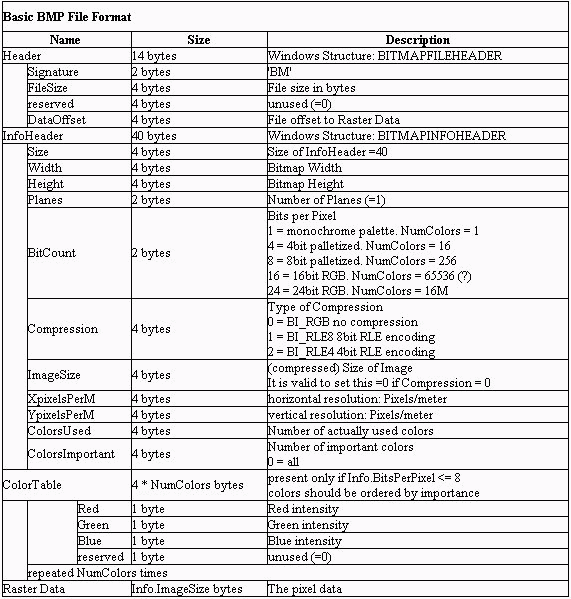
\includegraphics[width=\linewidth]{media/bmp_header.png}
\end{figure}
\break

\subsection{Cabeçalho de Arquivo}

O cabeçalho de arquivo possui 14 bytes de tamanho, como descrito na imagem acima.

\begin{center}
\begin{tabular}{|p{0.2\linewidth}|p{0.1\linewidth}|p{0.6\linewidth}|}
    \hline
    \textbf{Campo} & \textbf{Bytes} & \textbf{Descrição}\\
    \hline
    Validação & \textbf{2 bytes} & É usado para a validação do formato, seria seu magic number, geralmente é preenchido com "BM".\\
    \hline
    Tamanho & \textbf{4 bytes} & Tamanho do arquivo em bytes.\\
    \hline
    Reservado & \textbf{4 bytes} & Geralmente não é utilizado.\\
    \hline
    Offset & \textbf{4 bytes} & A partir de onde podemos começar a ler os dados dos pixels do arquivo. Em uma imagem padrão, que não tenha informações extra antes dos pixels, esse valor é 54 geralmente, que seria a soma dos valores de ambos os cabeçalhos (14 + 40).\\
    \hline
\end{tabular}
\end{center}

Poderia representá-lo assim em C.
\begin{lstlisting}[language=C, caption=Cabeçalho de Arquivo em C]
struct FileHeader {
    char magic[2];
    char size[4];
    char reserved[4];
    char offset[4];
};
\end{lstlisting}

\subsection{Cabeçalho de Informação}

O cabeçalho de informação tem 40 bytes de tamanho, e é nele que geralmente vão as informações relativas a imagem como sua paleta de cores, a quantidade de bits que estou usando para representar um pixel, as dimensões, entre outras coisas.
\begin{center}
\begin{tabular}{|p{0.2\linewidth}|p{0.1\linewidth}|p{0.6\linewidth}|}
    \hline
    \textbf{Campo} & \textbf{Bytes} & \textbf{Descrição} \\
    \hline
    Tamanho do Cabeçalho & \textbf{4 bytes} & Aqui irá conter o tamanho do cabeçalho em bytes, geralmente esse valor será 40 mesmo.\\
    \hline
    Largura & \textbf{4 bytes} & Largura da imagem\\
    \hline
    Altura & \textbf{4 bytes} & Altura da imagem\\
    \hline
    Planos & \textbf{2 bytes} & Número de planos (também não sei para que serve, geralmente é 1)\\
    \hline
    Bits Por Pixel & \textbf{2 bytes} & Esse campo é interessante, nele eu especifico a quantidade de bits que quero usar para representar um pixel. É comum esse valor ser 24 (RGB com 3 bytes, ou seja 1 byte para cada canal) ou 32 (RGBA com 4 bytes). Porém também pode ser 16 (também é RGB, mas é um RGB565, 5 bits para R, 6 para G e 5 para B). Se setarmos valores abaixo de 16, como 8 ou 4, precisamos especificar uma paleta de cores logo depois do cabeçalho. 8 bits por exemplo, preciso de uma paleta com 256 cores, 4 bits uma paleta com 16 cores e assim vai.\\
    \hline
    Compressão & \textbf{4 bytes} & Aqui basicamente você pode setar um modo de compressão, mas como não estamos utilizando nenhum geralmente esse valor será zero mesmo.\\
    \hline
    Tamanho da Imagem & \textbf{4 bytes} & Aqui vai representar o tamanho da imagem após a compressão. Se não tiver nenhuma compressão, como é o nosso caso, esse valor pode ser zero também.\\
    \hline
    
\end{tabular}
\end{center}

\begin{center}
\begin{tabular}{|p{0.2\linewidth}|p{0.1\linewidth}|p{0.6\linewidth}|}
    \hline
    XpixelsPerM & \textbf{4 bytes} & \\
    \hline
    YpixelsPerM & \textbf{4 bytes} & \\
    \hline
    Cores Usadas & \textbf{4 bytes} & \\
    \hline
    Cores Importantes & \textbf{4 bytes} & \\
    \hline
\end{tabular}
\end{center}

Posso representar esse cabeçalho assim em C:
\begin{lstlisting}[language=C, caption=Cabeçalho de Informação em C]
struct InfoHeader {
    char header_size[4];
    char width[4];
    char height[4];
    char planes[2];
    char bits_per_pixel[2];
    char compression[4];
    char image_size[4];
    char x_pixels[4];
    char y_pixels[4];
    char colors_used[4];
    char colors_important[4];
};
\end{lstlisting}

\section{Criando um Bitmap em C}

Agora vamos botar um pouco a mão na massa, vamos escrever um programinha em em C que fazendo uso dos cabeçalhos consiga fazer uma imagem bitmap que possamos visualizar em qualquer editor/visualizador de imagens.
\newpage

\begin{lstlisting}[language=C, caption=Cabeçalhos]
#include <stdio.h>

struct __attribute__((__packed__)) FileHeader {
    short magic;
    int size;
    int reserved;
    int offset;
};

struct __attribute__((__packed__)) InfoHeader {
    int size;
    int width;
    int height;
    short planes;
    short bits_per_pixel;
    int compression;
    int image_size;
    int x_pixels;
    int y_pixels;
    int colors_used;
    int colors_important;
};
\end{lstlisting}

Aqui estou me aproveitando alguns recursos do compilador, o\\ \_\_attribute\_\_((\_\_packed\_\_))  serve para ele tentar comprimir meu formato de maneira a evitar bytes vazios entre os campos.
Se eu não tivesse feito isso, entre os campos de \textbf{magic} e \textbf{size} do meu FileHeader, iriam existir dois bytes extras, então no fim meu struct teria 16 bytes de tamanho. Mas como nesse caso cada byte faz diferença, eu pedi para o compilador evitar fazer isso pois preciso preservar os 14 bytes.
Fique atento pois dependendo do compilador que você estiver usando pode ser que isso não funcione.

Agora vamos usar isso para criar nossa imagem. Vou criar uma imagem pequena para facilitar a explicação, terá dimensões 2x2 e com formato RGB.
Isso quer dizer que nossa imagem terá no total 4 pixels, e se cada pixel tem 3 bytes de tamanho, então no fim terei 12 bytes de dados. Porém o formato bitmap exige que você preencha cada linha com 1 byte extra para cada pixel para manter o alinhamento de 4 bytes para cada um. Outro detalhe importante é que os pixels quando escritos no documento são escritos ao contrário, então fica BGR, no fim terei algo assim: $BGR\ BGR\ 0 0$. Considerando os bytes extras, meus dados terão 16 bytes de tamanho, somando isso ao cabeçalho, terei um arquivo de 70 bytes de tamanho.

Vamos tentar escrever isso.
\begin{lstlisting}[language=C, caption=Escrevendo um Bitmap]
int main(int argc, char** argv) {

    FileHeader fh;
    InfoHeader ih;

    fh.magic = 0x4D42; // M(4D) B(42)
    fh.size = 70; // 70 bytes
    fh.offset = 54;

    ih.size = 40;
    ih.width = 2;
    ih.height = 2;
    ih.planes = 1;
    ih.bits_per_pixel = 24;
    ih.compression = 0;
    ih.image_size = 0;
    ih.x_pixels = 0;
    ih.y_pixels = 0;
    ih.colors_used = 0;
    ih.colors_important = 0;

    FILE* fp = fopen("image.bmp", "wb");

    fwrite(&fh, 1, sizeof(fh), fp);
    fwrite(&ih, 1, sizeof(ih), fp);

    char data[16] = {
    // |b    |g    |r   ||b    |g    |r    |extra bytes
        0x00, 0x00, 0xff, 0x00, 0xff, 0x00, 0x00, 0x00,
        0xff, 0x00, 0x00, 0xff, 0xff, 0xff, 0x00, 0x00,
    };

    fwrite(data, 1, sizeof(data), fp);
    fclose(fp);

    return 0;
}
\end{lstlisting}

E no fim, essa é a imagem que nós acabamos de criar:
\begin{figure}[h]
    \centering
    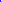
\includegraphics[width=5cm]{media/image.png}
    \caption{Imagem Gerada}
\end{figure}
\break

Agora perceba que os dados que escrevemos é diferente do resultado final da imagem.
Nós escrevemos vermelho (0 0 255 em BGR) x verde (0 255 0) na primeira linha, e azul (255 0 0 BGR) x branco (255 255 255) na segunda. Porém a imagem saiu o exato oposto, a primeira linha é azul x branco e a segunda vermelho x verde. Isso acontece porque as linhas são lidas de baixo para cima.
Ou seja, dos nossos 16 bytes de dados, é lido primeiro os últimos 8 bytes (0xff 0x00 0x00 | 0xff 0xff 0xff | 0x00 0x00), e aí sim os primeiros 8 bytes (0x00 0x00 0xff | 0x00 0xff 0x00 | 0x00 0x00).
Isso é importante para entender o próximo tópico, que é como nós podemos criar um programa que consiga exibir imagens que estejam no formato bitmap.

\section{Lendo e Exibindo um Bitmap}

Para esse exemplo irei utilizar a biblioteca SDL2, que é uma framework que me permite criar uma janela e desenhar nela, fora input, áudio e outras funcionalidades. Recomendo você dar uma olhada com calma nela depois, eu gosto dela principalmente pelo suporte multiplataforma.

\end{document}